\chapter{State of the Art on Zero-Knowledge Friendly Hash Functions}
\label{sec:zk-hashes}
This chapter will provide a theoretical approach of the hash functions that will be implemented.

\section*{Overview}
Most of the hash functions that work in zero-knowledge operate within a finite field, with their efficiency usually related to the number of multiplications and additions in the circuit.
Traditional hash functions such as SHA-256 or AES are designed to operate on bits and perform bitwise operations. However, when these bit-oriented hash functions are used in zero-knowledge proofs, they often result in very large circuit sizes, reducing efficiency. This inefficiency is due to the need for representing bitwise operations of long bit-size numbers, which usually involve numerous multiplications and additions within the circuit.

To address these issues, Arithmetization-Oriented (AO) hash functions have been developed. These hash functions are designed specifically for zero-knowledge proofs and operate within a finite field. By focusing on arithmetic operations rather than bitwise operations, AO hash functions simplify the circuit complexity. Consequently, they enable more efficient computations in zero-knowledge proofs.

Moreover, some techniques will be introduced to minimize the number of multiplications in the zero-knowledge circuits for better efficiency.


\section{MiMC}
The first hash funcion we explain is MiMC~\cite{albrecht2016mimc}, it was publiched by Albrecht et al. in 2016 and designed to provide high performance for the applications of zero-knowledge proofs, Fully-Homomorphic Encryption (FHE) and Multi-Party-Computation (MPC) frameworks. This hash function is very simple, its core non-linear component is the function $F(x) := x^3$ that is iterated with subkey additions. The advantatge of using this function is that only requires two field multiplications, in contrast to using a look-up table S-box, which can be expensive to represent in an arithmetic circuit, for example.\\
MiMC provides three cryptographic primitives. First, we are going to describe the block cipher and finally a permutation. We consider MiMC just for cipher/permutation, and GMiMC~\cite{cryptoeprint:2019/397} or Hades~\cite{10.1007/978-3-030-45724-2_23} for hashing. All these primitives work in a finite field $\mathbb{F}_q$, where $q$ is a prime $p$ or a power of 2. In this thesis we will focus on $q=p$.

\subsection*{Block cipher}
First of all we are going to explain the block cipher, MiMC-$b/k$ is a keyed permutation where each input block is maped to a unique output block with $b$ as block size and $k$ as key size.

\subsubsection*{MiMC-p/p}
The MiMC block cipher takes an input $x \in F_{p}$ and does $r$ iterations over a round function. The round function consists on a key addition of the $k$ vector, the addition of a round constant $c_i \in F_{p}$ and the previous discussed non-linear function $F(x) := x^d$ for $x \in F_{p}$ is applied for updating the current sate. Additionally, we need to assure that $d\geq3$ is the smallest
permutation, so gcd$(d,p-1)=1$, explained in section~\ref{sec:s-box}.\\
The encryption function consists in $r$ iterations over the round functions, adding the key $k$ after $r$ rounds have been performed.\\
So, the round function is defined as 
\begin{equation}
    F_i(x) = F\left(x \oplus k \oplus c_i\right)
\end{equation}
and the encryption function is expressed as
\begin{equation}
    E_k(x) = \left(F_{r-1} \circ F_{r-2} \circ \dots F_0\right)(x) \oplus k
\end{equation}

Figure~\ref{fig:mimc-enc-img} represents the encryption process of MiMC for $d=3$.

The equation for calculating the number of rounds is
\begin{equation}
    r = \left\lceil\frac{p}{\log_2 3}\right\rceil
\end{equation}

The values of the $r - 1$ round constants can be choosen randomly from the field $\mathbb{F}_{p}$ except for the first $c_0$ and last $c_r$ round constant whose values are 0.

\begin{figure}[h]
    \centering
    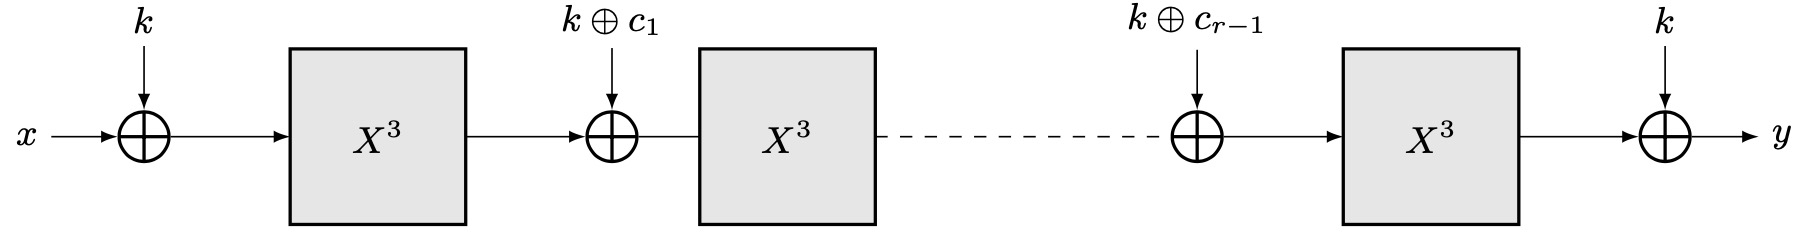
\includegraphics[width=\textwidth]{graphics/enc_mimc.jpg}
    \caption{Encryption process of MiMC~\cite{albrecht2016mimc} for $d=3$}
    \label{fig:mimc-enc-img}
\end{figure}

\subsubsection*{MiMC-2p/p}
In addition to the standard version of MiMC, there are some other variants, including those using a Feistel network, with extended key size, and using different round functions.
We focus on the \textbf{Feistel network} variant over prime fields, MiMC-$2p/p$. By using the Feistel network in the block cipher, we can process larger blocks, with two blocks being processed in each round.\\ 
The new round function of MiMC-$2p/p$ differs from the one in MiMC-$p/p$, taking the form~\cite{albrecht2016mimc}:
\begin{equation}
    x_L\|x_R \longleftarrow x_R \oplus \left(x_L \oplus k \oplus c_i\right)^3\|x_L
\end{equation}
However, the encryption function is the same as in MiMC-$n/n$.\\
In the Feistel network the round constants $c_i$ are also randomly generated from the $\mathbb{F}_{p}$ field. The cost for processing larger blocks comes with the incress of the number of rounds, where

\begin{equation}
    r' = 2 \cdot r = 2 \cdot \left\lceil\frac{p}{\log_2 3}\right\rceil
\end{equation}

Here, $r$ is the number of rounds of MiMC-$p/p$. Figure~\ref{fig:feistel-network} represents the encryption process of MiMC-$2p/p$. Because there is one more XOR operation and the number of rounds needs to be doubled, the computation of the encryption will be slightly slower than the regular MiMC.

\begin{figure}[htbp]
    \centering
    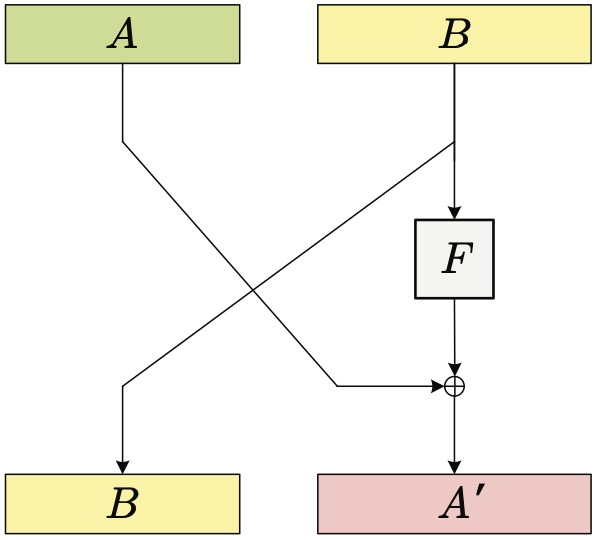
\includegraphics[width=0.4\textwidth]{graphics/feistel.jpg}
    \caption{Feistel network}
    \label{fig:feistel-network}
\end{figure}

\subsection*{MiMC permutation}
The MiMC permutation, MiMC$^P$, is obtained by setting all the key $k$ values to 0.

\section{Poseidon}
\label{sec:poseidon}
The Poseidon hash function~\cite{grassi2021poseidon}, published by Grassi et al. in 2021 works using the Poseidon$^\pi$ permutation within the sponge framework. This permutation is based on the Hades design, which will be explained below.
The hash function takes inputs from the $\mathbb{F}_{p}$ field, where $p$ is a prime number, and maps them to a fixed-length output over the $\mathbb{F}_{p}$ field, $\mathbb{F}_{p}^*\longrightarrow\mathbb{F}_{p}^o$, with $o$ representing the length of the output.

\subsection*{Hades strategy}
The Hades strategy doesn't use $r$ number of rounds, instead, it uses $r_f$ rounds initially, with full S-box layers. Subsequently, after these $r_f$ rounds, $r_p$ rounds are applied, but with only a single S-box. Finally $r_f$ rounds are applied again at the end, using full S-box layers.

Figure~\ref{fig:hades-enc-img} represents this explained aproach.\\
\begin{figure}[htbp]
    \centering
    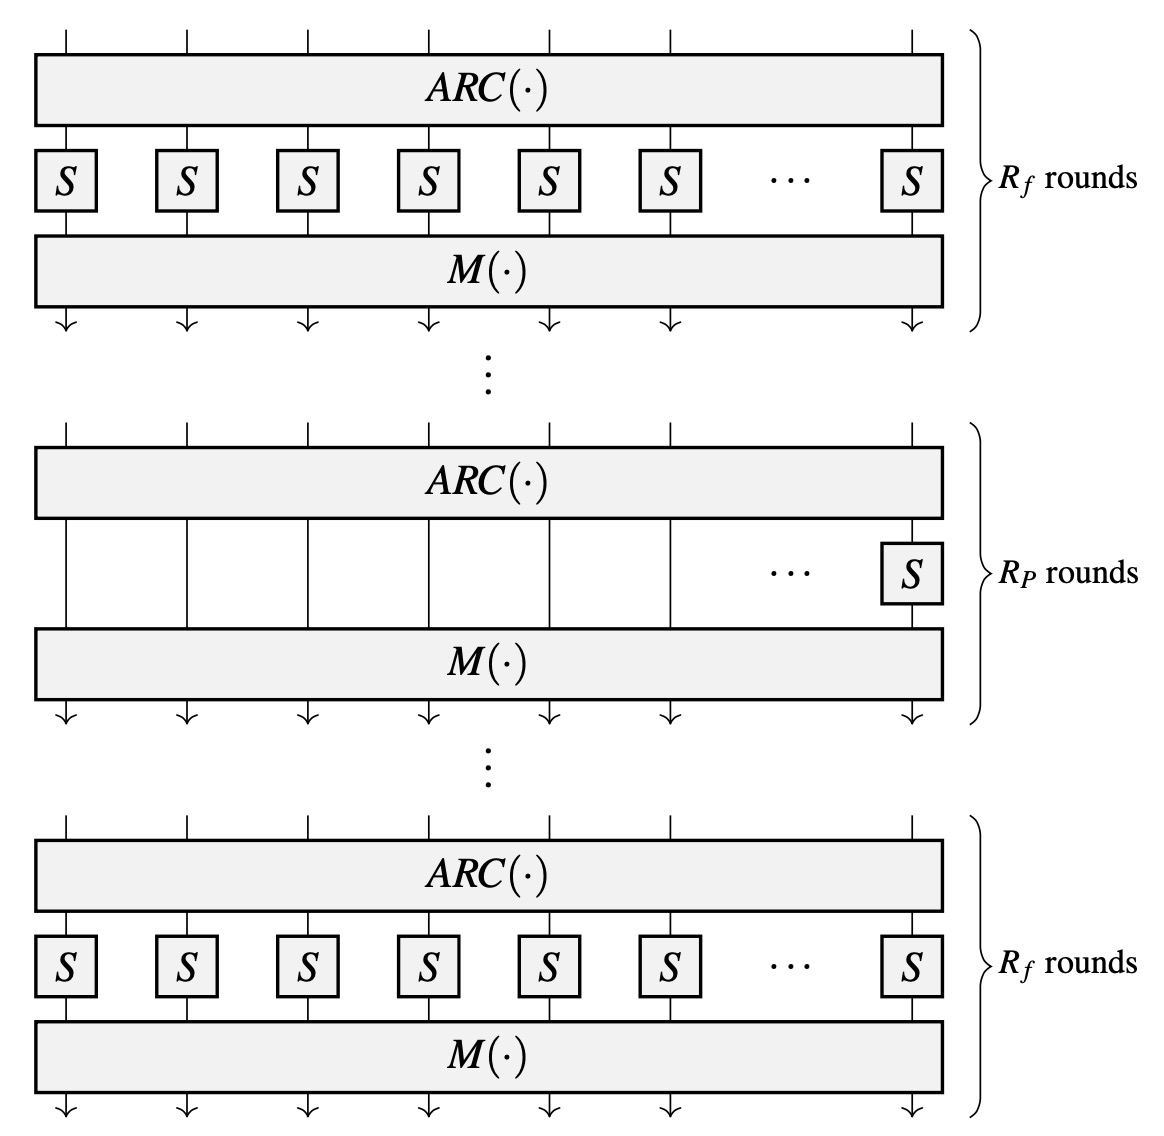
\includegraphics[width=0.8\textwidth]{graphics/hades_enc.jpg}
    \caption{Encryption process of Hades~\cite{grassi2021poseidon}}
    \label{fig:hades-enc-img}
\end{figure}

\subsubsection*{Poseidon round function}
The Poseidon round function is composed of two different rounds: full rounds and partial rounds.
The full round $\mathcal{E}$ is defined as
\begin{equation}
    \mathcal{E}_i(x) = M\cdot\left(\left(x_0+c_0^{(i)}\right)^d,\dots,\left(x_{t-1}+c_{t-1}^{(i)}\right)^d\right)
\end{equation}
for $i \in \{0,1,\dots,R_{r_f}-1\}$. The partial round $\mathcal{I}$ is defined as
\begin{equation}
    \mathcal{I}_i(x) = M\cdot\left(\left(x_0+c_0^{(i)}\right)^d,x_1+c_1^{(i)},\dots,x_{t-1}+c_{t-c}^{(i)}\right)
\end{equation}

for $i \in \{0,1,\dots,R_{r_p}-1\}$.

Table~\ref{tab:pos-round} represents the three steps of one round of Poseidon$^\pi$
\begin{table}[htbp]
    \centering
    \begin{tabular}{rl}
        \toprule
        & Hades round function \\
        \midrule
        1 & Add the round constants, denotated by $ARC(\cdot)$ \\
        2 & Apply substitution \\
        & i.  Full S-box$(\cdot)$ for $r_f$ rounds \\
        & ii. Partial S-box$(\cdot)$ for $r_p$ rounds \\
        3 & Multiply state with the MDS matrix, denotated by $M(\cdot)$ \\
    \end{tabular}
    \caption{One round of the Poseion$^\pi$}
    \label{tab:pos-round}
\end{table}

Next, we will describe the components of the Poseidon round function.

\subsubsection*{Constant layer}
The ARC($\cdot$) consists in adding the round constants $c_i$ to the state, where each component of the state will have a round constant added.

\subsubsection*{S-box layer}
The s-box layer is defined as Sbox$(x) = x^d$, where $d \geq 3$ is the smallest integer that satisfies $gcd(d,p-1) = 1$. For rounds without an S-box ($r_p$ rounds), the state remains unchanged and is forwarded as it is to the next round.

\subsubsection*{Linear layer}
The $t\times t$ Matrix with elements in $\mathbb{F}_{p}$ is a Maximum Distance Separable (MDS) matrix, which guarantees that each state component depends on each other component in each round. All $t$ components of the state will be multiplied by the $t \times t$ MDS matrix. The result of this multiplications is the input state for the next round layer. Unlike the Hades strategy, the linear layer is omitted in the last round.

\subsection*{Poseidon permutation}
The Poseidon$^\pi$ permutation over the vector space $\mathbb{F}_p^t$, where $t \geq 2$ is the length of the sponge state, is defined by
\begin{equation}
    \mathcal{P}(x) = \mathcal{E}_{R_F-1} \circ \dots \circ \mathcal{E}_{R_F/2} \circ \mathcal{I}_{R_P-1} \circ \dots \circ \mathcal{I}_0 \circ \mathcal{E}_{R_F/{2-1}} \circ \dots \circ \mathcal{E}_0(x),
\end{equation}
\label{eq:poseidon-perm}
where $\mathcal{E}$ represents a full round of the $R_F$ rounds and $\mathcal{I}$ is a partial round of $r_P$ rounds, with $R_F = 2\cdot r_f$.

\subsection*{Poseidon hash}
The Poseidon hash operates within the sponge construction, in the vector space $\mathbb{F}_p^{r+c}$, where $r$ is the rate and $c$ is the capacity of the sponge.

\section{Poseidon2}
The Poseidon2 hash function~\cite{grassi2023poseidon2} published by Grassi et al. in 2023, works within the sponge construction, being a more efficient version of Poseidon$^\pi$. Below, we explain the Poseidon2 hash, the Poseidon2 permutation and his round function.

\subsection*{Poseidon2 round function}
Similar to Poseidon, the Poseidon2 round function consists on two different rounds, a full round and a partial round.\\
The full round, $\mathcal{E}$, is defined as
\begin{equation}
    \mathcal{E}_i(x) = M_{\mathcal{E}}\cdot\left(\left(x_0+c_0^{(i)}\right)^d,\left(x_1+c_1^{(i)}\right)^d,\dots,\left(x_{t-1}+c_{t-c}^{(i)}\right)^d\right)
\end{equation}
where $d$ is the exponent of the S-box, and $c_j^{(i)}$ the j-th round constant in the i-th full round.\\
The partial round $\mathcal{I}$ is defined as
\begin{equation}
    \mathcal{I}_i(x) = M_{\mathcal{I}}\cdot\left(\left(x_0+\hat{c_0}^{(i)}\right)^d,x_1,\dots,\left(x_{t-1}\right)\right)
\end{equation}
where $d$ is the same exponent as before, and $\hat{c}_0^{(i)}$ is the round constant in the i-th partial round.\\
A description of the components used in the Poseidon2 round function is provided below.

\subsubsection*{Constant layer}
The round constants are generated as in Poseidon$^\pi$.

\subsubsection*{Linear layer}
Firstly, the case of $t = 4t' \geq 4$ is considered, followed by $t\in\{2,3\}$.
For the \textbf{full rounds} and $t = 4t'$ with $t' \in \mathbb{N}$, the matrix is defined as
\begin{equation}
    M_\mathcal{E} =
    \begin{cases}
        M_4 & \text{if } t=4, \\
        \text{circ}\left(2\cdot M_4,M_4,\dots,M_4\right)\in \mathbb{F}_p^{t\times t} & \text{if } t\geq 8,
    \end{cases}
\end{equation}
where $M_4$ is a $4\times 4$ MDS matrix
\begin{equation}
    M_4 = 
    \begin{pmatrix}
        5 & 7 & 1 & 3 \\
        4 & 6 & 1 & 1 \\
        1 & 3 & 5 & 7 \\
        1 & 1 & 4 & 6
    \end{pmatrix}
    ,
\end{equation}

An efficient way for computing vector per matrix multiplication is defined in~\cite{duval2018mds}. Corresponding to the $M_{4,4}^{8,4}$ matrix, with $\alpha = 2$.

For the \textbf{partial rounds}, the MDS matrix is no longer necessary. In this case, the matrix $M_\mathcal{I}$ is defined as
\begin{equation}
    M_{\mathcal{I}} = 
    \begin{pmatrix}
        \mu_0 & 1 & \dots & 1 \\
        1 & \mu_1 & \dots & 1 \\
        \vdots & \vdots & \ddots & \vdots \\
        1 & 1 & \dots & \mu_{t-1}
    \end{pmatrix}
    ,
\end{equation}

where $\left(\mu_0,\mu_1,\dots,\mu_{t-1}\right)$ are random elements from the field $\mathbb{F_p}\backslash\{0,1\}$.

\subsubsection*{Plonk Arithmetization}
For the partial round vector per matrix multiplication. Let's define a vector $\left(x_0,x_1,\dots x_{t-1}\right)$, the computation of the multiplication is
\begin{equation}
    \begin{cases}
        s = x_0,x_1,\dots ,x_{t-1}, \\
        y_i = \left(\mu_i-1\right)x_i+s & \text{for }i\in \{0,1,\dots,t-1\},
    \end{cases}
\end{equation}
where $s$ represents the sum of the elements of the vector and $y$ is the output vector.\\
Additionally, for $t\in\{2,3\}$, we set the condition that $M_\mathcal{I}$ is MDS, so, first $M_{\mathcal{I}}$ is computed and we set $M_{\mathcal{I}} = M_{\mathcal{E}}$. Appart from this we also check for
\begin{itemize}
    \item $t=2$ if $\mu_0\mu_1-1 \neq 0$ and $\mu_0,\mu_1 \neq 0$,
    \item $t=3$ if $\mu_0\mu_1\mu_2-\mu_0-\mu_1-\mu_2 \neq 0$ and
        $\mu_0\mu_1\mu_2\neq0,$  $\mu_0\mu_1-1\neq0,$ $\mu_0\mu_2-1\neq0,$ $\mu_1\mu_2\neq0$.
\end{itemize}

\subsubsection*{S-box layer}
The S-box layer is defined as Sbox$(x) = x^d$, where $d\geq3$ is the smallest positive integer such that gcd$\left(d,p-1\right)=1$.

\subsection*{Poseidon2 permutation}
The permutation is defined over the $\mathbb{F}_p^t$ vector space, where $p$ is a prime number and $t \in \{2,3,4,\dots,4\cdot t',\dots,24\}$ is the length of the state of the sponge for $t' \in \mathbb{N}$. The Poseidon2$^\pi$ is defined as
\begin{equation}
    \mathcal{P}_2(x) = \mathcal{E}_{R_F-1} \circ \dots \circ \mathcal{E}_{R_F/2} \circ \mathcal{I}_{R_P-1} \circ \dots \circ \mathcal{I}_0 \circ \mathcal{E}_{R_F/{2-1}} \circ \dots \circ \mathcal{E}_0(M_{\mathcal{E}\cdot}x)
\end{equation}
where $\mathcal{E}$ is the full round and $\mathcal{I}$ is the partial round, whith the same number of rounds as in Equation~\ref{eq:poseidon-perm} of Poseidon$^\pi$.

\subsection*{Poseidon2 hash}
Similar to the other hash functions presented in this thesis, the Poseidon2 hash also operates within a sponge construction in the field $\mathbb{F}_p^{r+c}$, where $r$ is the rate and $c$ the capacity of the sponge.

\subsection*{Poseidon$^\pi$ vs Poseidon2$^\pi$}
The differences between the permutation of Poseidon2 and Poseidon are provided below. Figure~\ref{fig:poseidon-vs-2} shows a visual representation of these difference.
\begin{itemize}
    \item The linear layer is also applied at the input of the permutation.
    \item Two diferent linear layers are used for $t\geq4$.
    \item In each round only one round function is applied.
\end{itemize}

\begin{figure}[htbp]
    \centering
    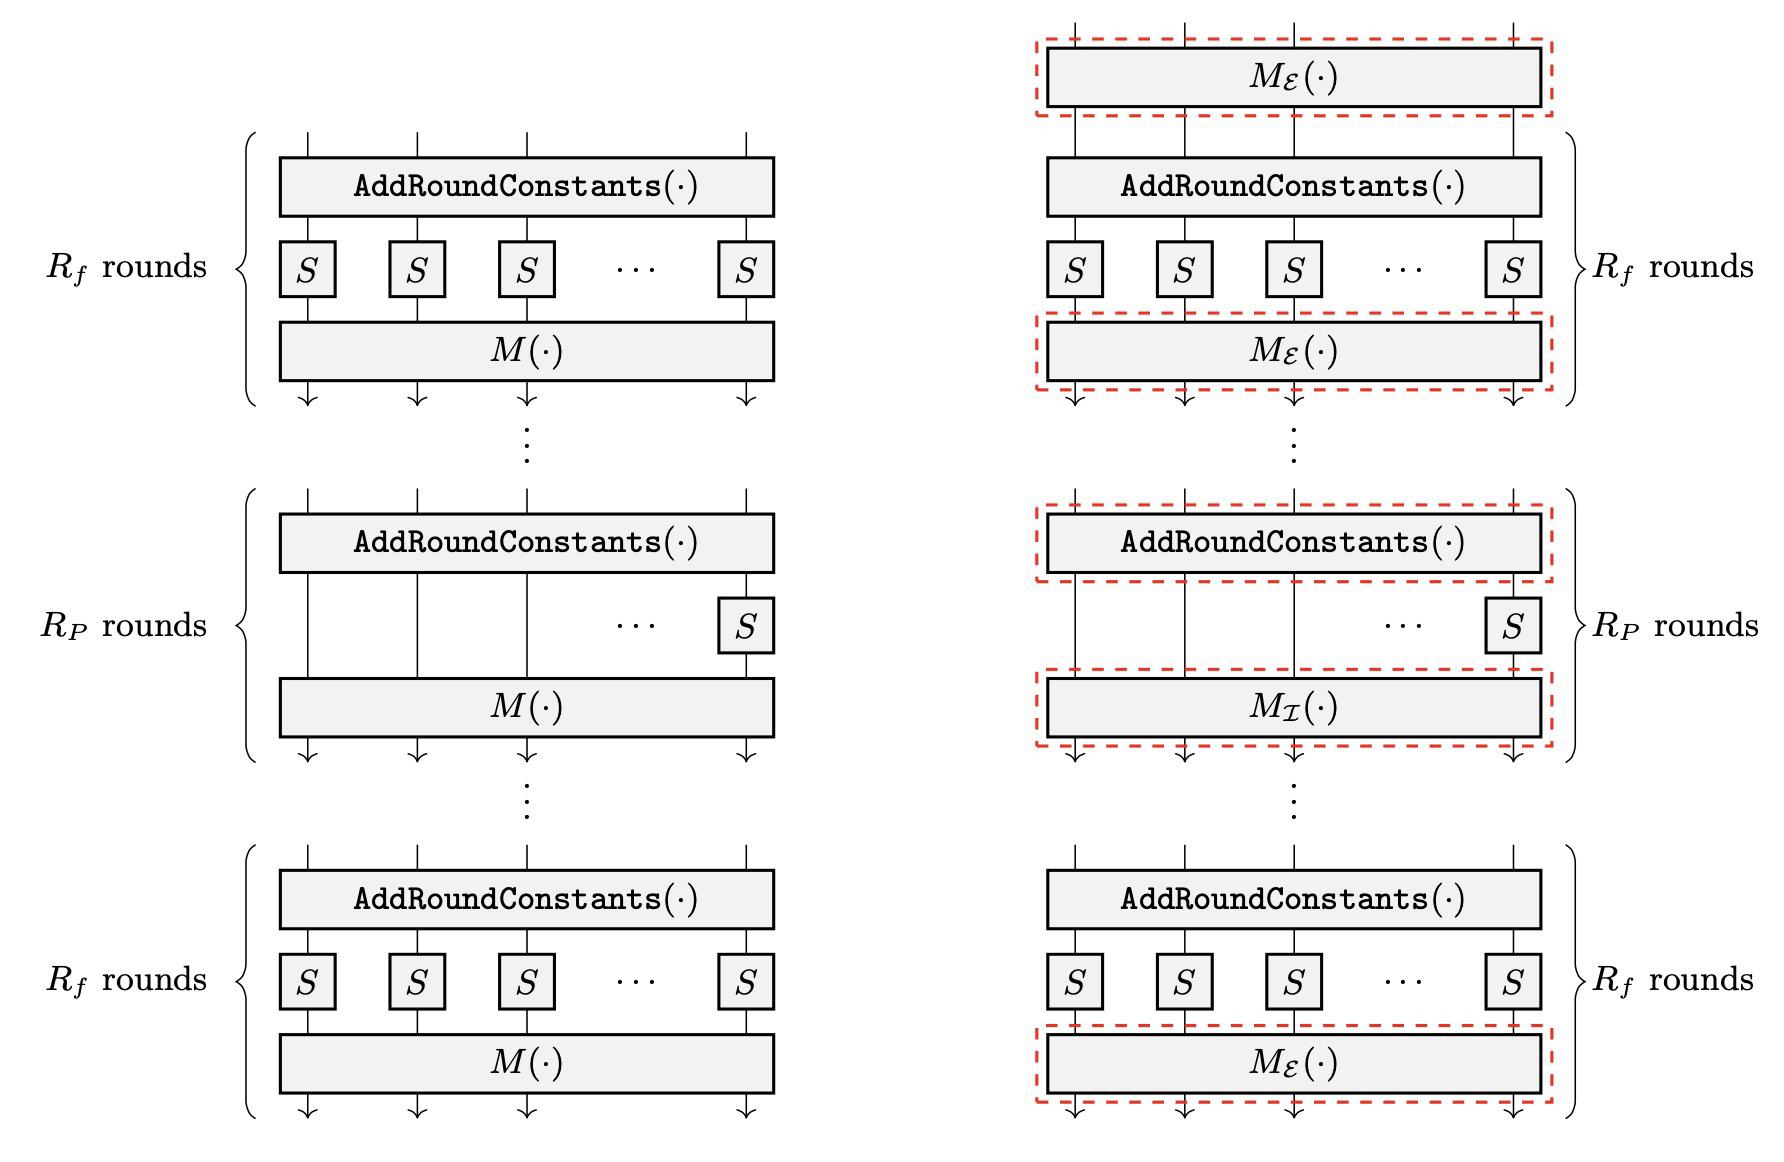
\includegraphics[width=\textwidth]{graphics/poseidon_vs_poseidon2.png}
    \caption{Poseidon$^\pi$ vs Poseidon2$^\pi$~\cite{grassi2023poseidon2}}
    \label{fig:poseidon-vs-2}
\end{figure}

\section{Rescue-prime}
\label{sec:Rescue-prime}
Rescue~\cite{szepieniec2020rescue} published by Szepieniec et al. in 2020, operates on field elements on $\mathbb{F}_{p}$, where $p$ is a prime field, and the state is a vector in the vector space $\mathbb{F}_{p}^m$, where $m$ is the number of elements. Here, we will explain both the standard and the optimized versions of Rescue-prime.

\subsection*{Rescue round function}
The Rescue round function~\cite{aly2020design} operates over the vector space $\mathbb{F}_p^{m}$, where $p$ is a prime number.
Below, Table~\ref{tab:rescue-sing-round} presents the components and steps of a single round $i$, while Figure~\ref{fig:rescue-i-round} provides a diagram of it.


\begin{table}[htbp]
    \centering
    \begin{tabular}{rl}
        \toprule
        & Rescue round function \\
        \midrule
        1 & S-box layer, apply $(\cdot)$ to each element of the state. \\
        2 & Linear layer, matrix-vector multiplication of the MDS matrix and the state. \\
        3 & Constants layer, add from the list of round constants $\{C_i\}_{i=0}^{2mN-1}$, $m$ constants \\
        & to the state. \\
        4 & Inverse S-box layer, apply $(\cdot)^{\alpha^{-1}}$ to each element of the state. \\
        5 & Liner layer, matrix-vector multiplication of the MDS matrix and the state. \\
        6 & Constants layer, add from the list of round constants $\{C_i\}_{i=0}^{2mN-1}$, $m$ constants \\
        & to the state. \\
    \end{tabular}
    \caption{One round components}
    \label{tab:rescue-sing-round}
\end{table}

\begin{figure}
    \centering
    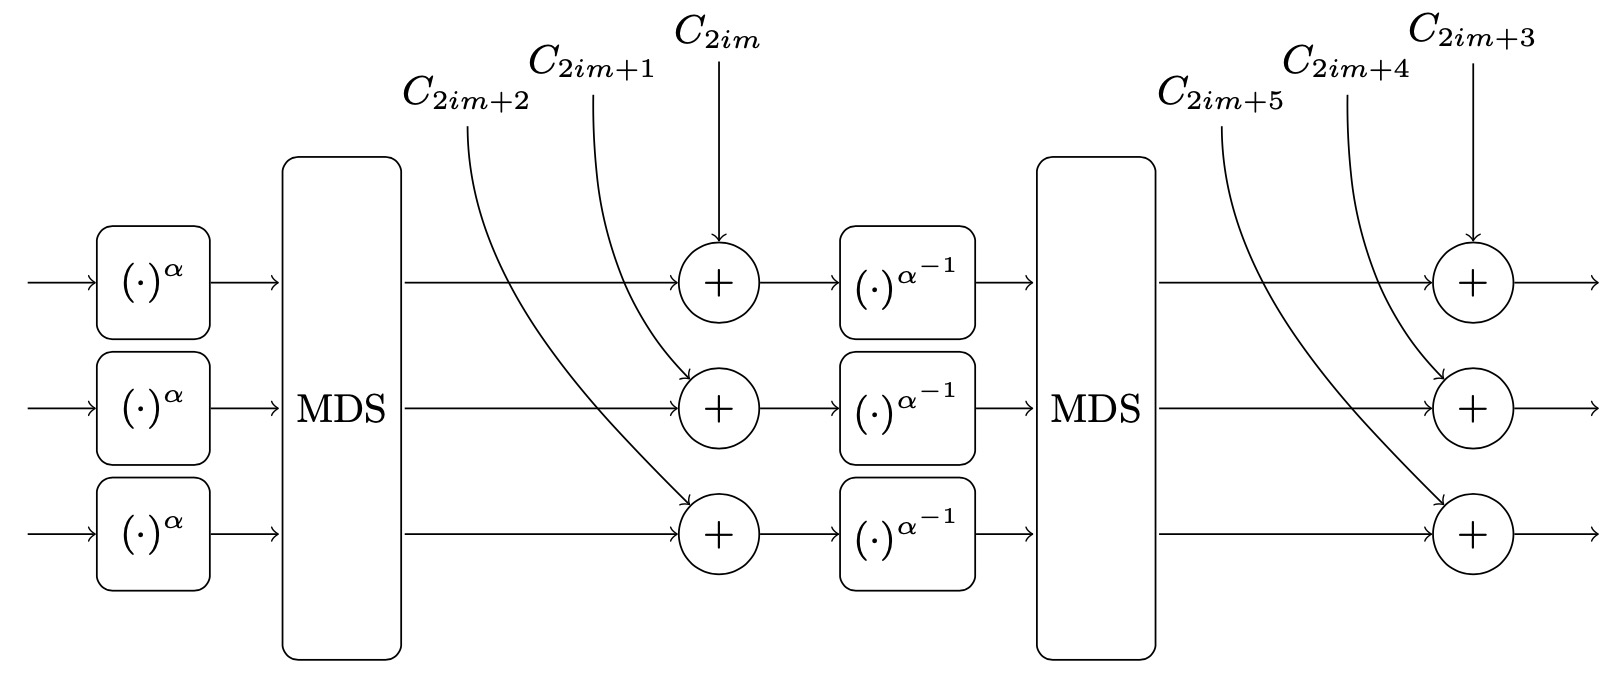
\includegraphics[width=0.9\textwidth]{graphics/rescue_i_round.jpg}
    \caption{Round $i$ of Rescue$^\pi$~\cite{szepieniec2020rescue}}
    \label{fig:rescue-i-round}
\end{figure}

To build the S-box, we find the smallest prime $\alpha$ such that $gcd(p-1, \alpha) = 1$. Therefore, the S-box is defined as $S : \mathbb{F}_{p} \longrightarrow \mathbb{F}_{p} : x \mapsto x^\alpha$ and $S^{-1} : \mathbb{F}_{p} \longrightarrow \mathbb{F}_{p} : x \mapsto x^{1/\alpha}$, where $1/\alpha$ is the multplicative inverse of a modulo $p-1$, whose existance is guaranteed by the fact that gcd$(\alpha, p - 1) = 1$. The generation of the MDS matrix and the round constants is out of the scope of this thesis, although~\cite{szepieniec2020rescue} provides a SageMath implementation with the computation of the number of rounds and the MDS matrix.

\subsection*{Rescue-prime optimized}
The optimized version of the Rescue-prime~\cite{ashur2022rescue} published in 2022, works only over the Goldilocks prime field, where $p = 2^{64} - 2^{32} + 1$, explained in section~\ref{sec:finite-fields}.

It uses the same components of the standard Rescue-prime round function, but the order of the operations differs from the standard version. The new order is presented in Table~\ref{tab:rescue-opt-round-comp}. 

\begin{table}[htbp]
    \centering
    \begin{tabular}{rl}
        \toprule
        & Rescue-prime optimized round function \\
        \midrule
        1 & MDS matrix \\
        2 & Constant layer \\
        3 & S-box layer \\
        4 & MDS matrix \\
        5 & Constant layer \\
        6 & Inverse S-box layer \\
        \bottomrule
    \end{tabular}
    \caption{Rescue-prime optimized single round components}
    \label{tab:rescue-opt-round-comp}
\end{table}

\subsubsection*{Parameters}
In the optimized version, certain parameters are fixed. The exponents of the S-box and the inverse S-box, $\alpha$ and $\alpha^{-1}$, are set to $\alpha = 7$ and $\alpha^{-1} = 10540996611094048183$. Table~\ref{tab:rescue-param-opt} provides additional parameters.

\begin{table}[htbp]
    \centering
    \begin{tabular}{cccc}
      \toprule
      Prime field $p$ & $2^{64} - 2^{32} + 1$  \\
      Number of rounds $N$  & 7   \\
      State size $m$       & 12   \\
      Rate $r$       & 8          \\
      Capacity $c$  & 4           \\
      \bottomrule
    \end{tabular}
    \caption{Integer parameters for the Rescue-prime optimization}
    \label{tab:rescue-param-opt}
  \end{table}

  \subsubsection*{MDS Matrix}
The MDS matrix is a circulant matrix with the first row defined as:
\[[7,23,8,26,13,10,9,7,6,22,21,8]\]

\subsubsection*{Overwrite mode}
In contrast to the standard Sponge construction, the elements from the state associated with the rate are added by the matching elements from the input chunk, but in this optimized case, the elements are not added but they are overwritten. In other words, if the $state[j]$ represents the state elements and $input[j]$ the input chunk, it will permorm this absorbing operation $state[j] \leftarrow input[j]$ instead of $state[j] \leftarrow state[j] + input[j]$ 

\subsubsection*{Indexing of state elements}
In the optimized version, the state is composed by the capacity and the rate, where each one indices from 0 to $c - 1$ and $c$ to $m - 1$, respectively.

\subsection*{Rescue-prime permutation}
The Rescue-prime permutation consists in iterating N times the round function.

\subsection*{Rescue-prime hash}
Both the standard and optimized versions of Rescue-prime utilize the Sponge construction for hashing.

\subsubsection*{Sponge construction}
There is a modification in the squeezing phase of the sponge construction and the one explained in section~\ref{sec:sponge-construction}. In the squeezing phase the top $r$ elements of the state are the output, note that we don't apply the permutation in this phase.

Figure~\ref{fig:rescue-prime-hash} demonstrate this modification for $N=2$.

\begin{figure}
    \centering
    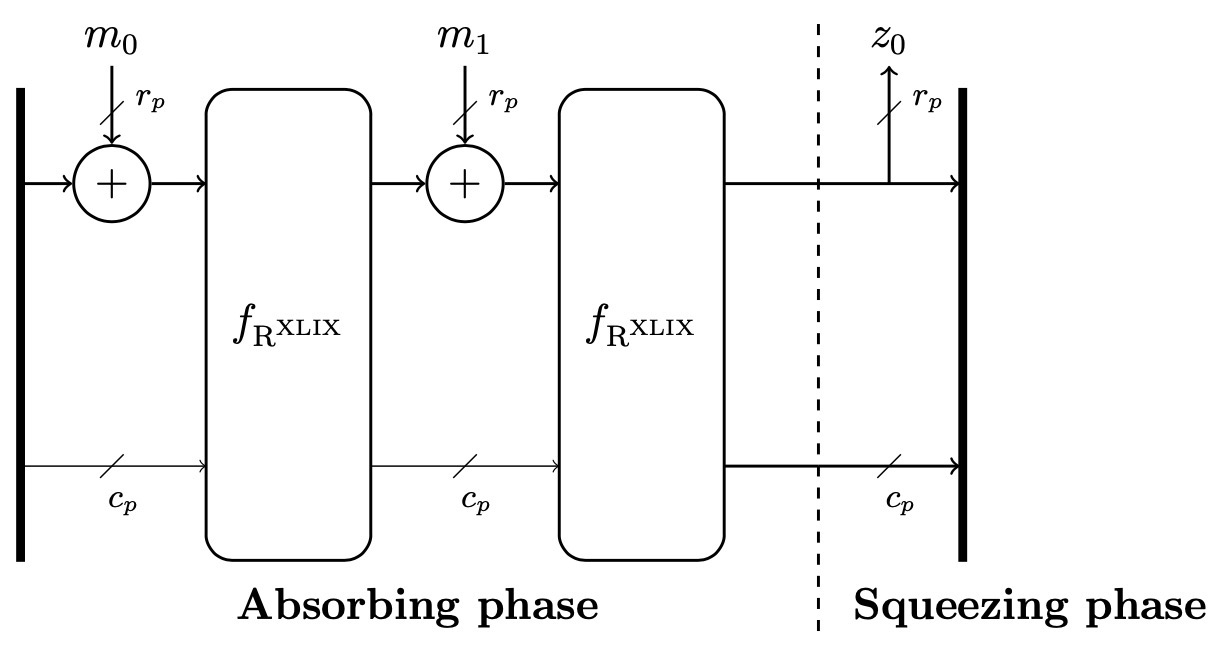
\includegraphics[width=0.7\textwidth]{graphics/rescue-prime-hash.png}
    \caption{Rescue-prime hash function with $N=2$~\cite{szepieniec2020rescue}}
    \label{fig:rescue-prime-hash}
\end{figure}

\section{Griffin}
\label{sec:griffin}
We are going to explain the Griffin hash function~\cite{grassi2022horst}, proposed by Grassi et al. in 2022. It is a hash function that operates over the permutation, Griffin$^\pi$, and a round function.

\subsection*{Griffin round function}
The Griffin round function, denoted as $\mathcal{F}_i$, is defined as
\begin{equation}
    \mathcal{F}_i(\cdot) = c^{(i)} + \mathcal{M} \times \mathcal{S}(\cdot).
\end{equation}
Here, $c^{(i)} \in \mathbb{F}_{p}^t$ is the round constant, where $c^{R-1} = 0$, $\mathcal{S} : \mathbb{F}_{p}^t \longrightarrow \mathbb{F}_{p}^t$ is a nonlinear layer, and $i \in \{0,1,\dots,R-1\}$ with $R$ being the number of rounds. The round constants that are added to the state will be different in every round but the matrix $M$ that is applied to the state will be the same in every round.\\
Each one of the components of the round function will be explained next.

\subsubsection*{Nonlinear layer \textit{S}}
The permutation is limited in $t \leq 24$, with $d$ taking values from $\{3,5,7,11\}$, similar to the previous hash functions. These values are choosen such that $gcd(d,p-1) = 1$. Additionally, $\alpha_i$ and $\beta_i \in \mathbb{F}_{p}^2 \backslash\{(0,0)\}$ are a pairwise distinct, ensuring that $\alpha_i^2 - 4\beta_i$ is a quadratic nonresidu modulo $p$ for $2\leq i \leq t-1$.\\
The nonlinear layer $\mathcal{S}(x_0,\dots,x_{t-1}) = y_0 \| \cdot\cdot\cdot\|y_{t-1}$ is composed of two nonlinear sublayers defined via three different nonlinear functions. Two of them are defined via the invertible power maps $x\mapsto x^d$ and $x\mapsto x^{1/d}$, inspired by Rescue. The final one uses the Horst scheme (Section~\ref{sec:horst}), using the map $(x,y)\mapsto(x,y\cdot G(x))$ for a quadratic function $G$ such that $G(z)\neq0$ for each $z$. It is defined as:
\begin{equation}
    y_i = \begin{cases}
        x_0^{1/d} & \text{if i } = 0, \\
        x_1^d & \text{if i } = 1, \\
        x_2 \cdot \left(\left(L_i\left(y_0,y_1,0\right)\right)^2 + \alpha_2 \cdot L_i\left(y_0,y_1,0\right)+ \beta_2\right) & \text{if i } = 2, \\
        x_i \cdot \left(\left(L_i\left(y_0,y_1,x_{i-1}\right)\right)^2 + \alpha_i \cdot L_i\left(y_0,y_1,x_{i-1}\right) + \beta_i\right) & \text{otherwise},  
    \end{cases}
\end{equation}
where $L_i : \mathbb{F}_{p}^3 \longrightarrow \mathbb{F}_{p}$ represents $L_i\left(z_0,z_1,z_2\right) = \gamma_i \cdot z_0 + z_1 + z_2$ for $\gamma_i \in \mathbb{F}_{p} \backslash \{0\}$.

\textbf{Linear layer \textit{M}}\\
For $t \in \{3,4\}$, the matrix $M$ must be MDS,
\begin{equation}
    M_3 = 
    \begin{pmatrix}
        2 & 1 & 1 \\
        1 & 2 & 1 \\
        1 & 1 & 2 
    \end{pmatrix}
    \text{, } M_4 = 
    \begin{pmatrix}
        5 & 7 & 1 & 3 \\
        4 & 6 & 1 & 1 \\
        1 & 3 & 5 & 7 \\
        1 & 1 & 4 & 6
    \end{pmatrix}
    \text{,}
\end{equation}

we can use the efficient method proposed in~\cite{duval2018mds} to compute the matrix per vector multiplication, where the $M_4$ corresponds to $M_{4,4}^{8,4}$, setting $\alpha = 2$.

When $t \geq 8$, $M$ is
\begin{equation}
    M = M'' \times M' \equiv M' \times M'' =
    \begin{pmatrix}
        2\cdot M_4 & M_4 & \dots & M_4 \\
        M_4 & 2\cdot M_4 & \dots & M_4 \\
        \vdots & \vdots & \ddots & \vdots \\
        M_4 & M_4 & \dots & 2\cdot M_4
    \end{pmatrix}
    ,
\end{equation}
where $M'=$ diag$\left(M_4,M_4,\dots,M_4\right) \in \mathbb{F}_{p}^{t\times t}$ and $M'' =$ circ$\left(2\cdot I, I,\dots,i\in \mathbb{F}_{p}^{t\times t}\right)$ and $M_4$ is a $4\times 4$ MDS matrix and $I$ is the $4\times 4$ identity matrix.

\subsection*{Griffin permutation}
The Griffin permutation, denotated as $\mathcal{G}^\pi : \mathbb{F}_{p}^t \longrightarrow \mathbb{F}_{p}^t$ is defined as
\begin{equation}
    \mathcal{G}^\pi(\cdot) := \mathcal{F}_{\mathcal{R}-1} \circ \mathcal{F}_1 \circ \mathcal{F}_0(\mathcal{M}\times \cdot),
\end{equation}
where $\mathcal{M}$ is a matrix defined as above, and $\mathcal{F}_i : \mathbb{F}_{p}^t \longrightarrow \mathbb{F}_{p}^t$ represents the round function of the $\mathcal{G}^\pi$ permutation.\\
Figure~\ref{fig:griffin-permutation} shows the $\mathcal{G}^\pi$ permutation, where $\boxplus$ represents the addition opeeration of two vectors in the field $\mathbb{F}_{p}^t$.

\subsection*{Griffin-Sponge hash function}
The Griffin hash function operates over a field $\mathbb{F}_{p}$, where $p$ is a prime number and $t\in \{3,4t'\}$ the length of the state for a positive integer $t' \in \{1,2,\dots,6\}$, that means that $t$ must be 3 or a multiple of 4. Additionally, due to the use of the sponge construction, the rate $r$ must satisfy $r \geq t/3$.\\
Figure~\ref{fig:griffin-hash} provides the Griffin-Sponge hash function, where $\oplus$ represents the addition operation of two vectors in the field $\mathbb{F}_{p}^r$ and $\mathcal{G}^\pi$ the Griffin permutation.

\begin{figure}[htbp]
    \centering
    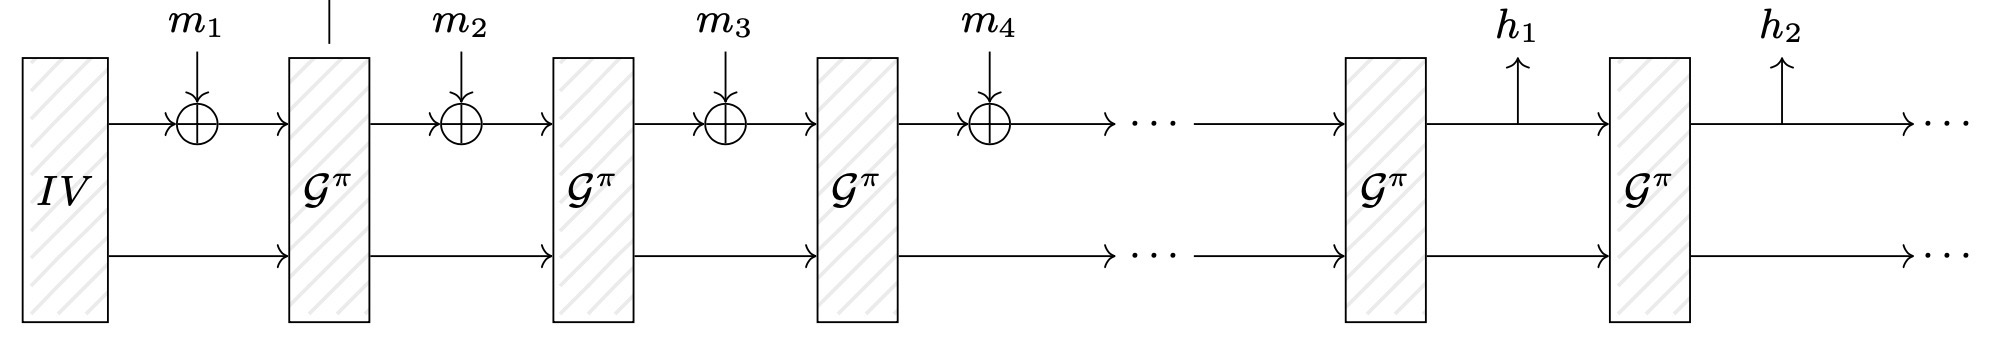
\includegraphics[width=\textwidth]{graphics/griffin-hash.png}
    \caption{Griffin-Sponge hash function~\cite{grassi2022horst}}
    \label{fig:griffin-hash}
\end{figure}

\begin{figure}[htbp]
    \centering
    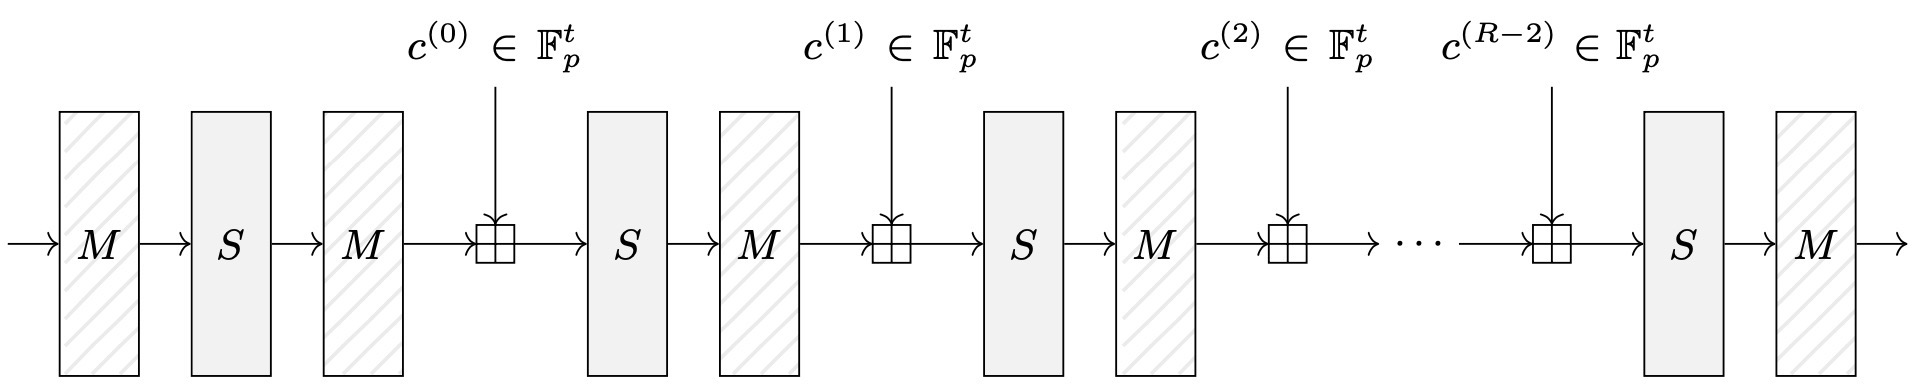
\includegraphics[width=\textwidth]{graphics/griffin-permutation.png}
    \caption{$\mathcal{G}^\pi$ permutation~\cite{grassi2022horst}}
    \label{fig:griffin-permutation}
\end{figure}

\section{Anemoi}
\label{sec:anemoi}
The Anemoi hash function~\cite{bouvier2023new} is also a very recent hash function, it was published by Bouvier et al. in 2023. It operates over a permutation, Anemoi$^\pi$, and this permutation works on a round function.\\
First we will start presenting the round function, next the permutation and finally the hash function.

\subsection*{Anemoi round function}
The Anemoi round function operates over the vector space $\mathbb{F}_q^{2l}$, where $l>0$, and $q$ is a prime number or a power of 2, in this thesis, we focus on $q=p$.

The length of the state is $2\times l$. In the Anemoi, the state is divided in two parts, the first part is $\left(x_0,\dots,x_{l-1}\right)$ and the second part is defined as $\left(y_0,\dots,y_{l-1}\right)$. We define a generator $g$ of the multiplicative subgrup of the field $\mathbb{F}_q$. If $q$ is prime, $g$ is the smallest generator, otherwiese $g$ is one of the roots of $\mathbb{F}_q = \mathbb{F}_{2^n}=\mathbb{F}_2[x]/p(x)$, where $p$ is an irreducible polynomial of degree $n$.

The structure of the Anemoi round function is composed of the following components: linear layer, S-box layer and constant addition. Figure~\ref{fig:anemoi-one-round} represents this structure.

Next, a description of each component is presented below.

\subsubsection*{Constant layer $\mathcal{A}$}
The constants layer corresponds to the addition of constants to the state vector, $x_j\leftarrow x_j+c_j^i$ and $y_j\leftarrow y_j+d_j^i$ where $c_j^i\in\mathbb{F}_q$ and $d_j^i\in\mathbb{F}_q$ are the round constants that depends on the position $i$ and the round $r$ of the permutation.\\
For calculating the round constants, we use
\begin{multline*}
    \pi_0=141592653589793238462643383279502884197169399375\\1058209749445923078164062862089986280348253421170679,
\end{multline*}
\begin{multline*}
    \pi_1=821480865132823066470938446095505822317253594081\\2848111745028410270193852110555964462294895493038196,
\end{multline*}
where $\pi_1$ and $\pi_2$ are the decimal expansion of $\pi$, and the computations for calculating the round constants $c_j^i$ and $d_j^i$ are
\begin{align}
    c_j^i=g\left(\pi_0^i\right)^2+\left(\pi_0^i+\pi_1^j\right)^\alpha \\
    d_j^i=g\left(\pi_1^j\right)^2+\left(\pi_0^i+\pi_1^j\right)^\alpha+g^{-1},
\end{align}

in the $\mathbb{F}_q$ field.

\subsubsection*{Linear layer $\mathcal{M}$}
In the Anemoi, the matrix M operates on the two vectors of the state $X=\left(x_0,\dots,x_{i-1}\right)$ and $Y=\left(y_0,\dots,y_{i-1}\right)$, separately. The matrix $M$ is defined as
\begin{equation}
    \mathcal{M}\left(X,Y\right)=\left(\mathcal{M}_x\left(X\right),\mathcal{M}_y\left(Y\right)\right),
\end{equation}
 $\mathcal{M}_x$ operates on the $X$ elements of the state and $\mathcal{M}_y$ on the $Y$ elements.\\
 We define $\mathcal{M}_x$ as a $l\times l$ matrix of $\mathbb{F}_q$ and $\mathcal{M}_y=\mathcal{M}_x\circ\rho$, where $\rho$ is a permutation over the $X$ vector defined as $\rho\left(x_0,\dots,x_{l-1}\right)=\left(x_1,\dots x_{l-1},x_0\right)$. The matrix $\mathcal{M}_x$ depends on the value of $l$. Depending on the $l$ size we separate two possible situations.
 \begin{itemize}
    \item $l$ is small, then the field size needs to be large.
    \item If $l$ is large, we expect a smallest field.
 \end{itemize}

 Similar to the previous hash functions, when $l \leq 4$ we can optimize the matrix and vector multiplications using the approach described in~\cite{duval2018mds}.\\
 In this cases, $l\in\{2,3,4\}$, the matrix $\mathcal{M}_x^l$ is
 \begin{equation}
    \mathcal{M}_x^2=
        \begin{pmatrix}
            1 & g \\
            g & g^2+1
        \end{pmatrix},\text{ }
    \mathcal{M}_x^3=
        \begin{pmatrix}
            g+1 & 1 & g+1 \\
            1 & 1 & g\\
            g & 1 & 1
        \end{pmatrix}, 
 \end{equation}
 \begin{equation}
    \mathcal{M}_x^4=
        \begin{pmatrix}
            1 & g^2 & g^2 & 1+g\\
            1+g & g+g^2 & g^2 & 1+2g \\
            g & 1+g & 1 & g \\
            g & 1+2g & 1+g & 1+g
        \end{pmatrix}.
 \end{equation}

 \subsubsection*{Pseudo-Hadamard transform $\mathcal{P}$}
 Anemoi uses a new layer that has not been used in the previous hash functions, it is used to increase the security after computing the S-box layer. It is very simple to implement, only needing two additions: $Y\leftarrow Y+X$ and $X\leftarrow X+Y$.
 
 \subsubsection*{Nonlinear layer $\mathcal{S}$}
 The nonlinear or S-box layer of the Anemoi also works different than in the previous hash functions. First we define the S-box as
 \begin{equation}
    \mathcal{S}\left(X,Y\right)=\left(\mathcal{H}\left(x_0,y_0\right),\dots,\mathcal{H}\left(x_{l-1,y_{l-1}}\right)\right),
 \end{equation}
where $\mathcal{H}$ is an \textit{open Flystel} (Section~\ref{sec:flyestel}) operating over $\mathbb{F}_q^2$. $\mathcal{H}$ uses 4 parameters, the exponent $\alpha$, the multiplier $\beta$, and the two constants $\gamma$ and $\delta$.\\
So, we let $\beta=g$, where $g$ has been defined before, $\delta\neq\gamma$, $\gamma=0$ and $\delta=g^{-1}$, and finally the exponent $\alpha$, that must satisfy gcd$\left(p-1,\alpha\right)=1$.

\begin{equation}
    \mathcal{H} = 
    \begin{cases}
        x_i\longleftarrow x_i-gQ(y_i)-g^{-1}\\
        y_i\longleftarrow y_i-x_i^{1/\alpha}\\
        x_i\longleftarrow x_i+Q(y_i)\\
    \end{cases}
\end{equation}

\begin{figure}[htbp]
    \centering
    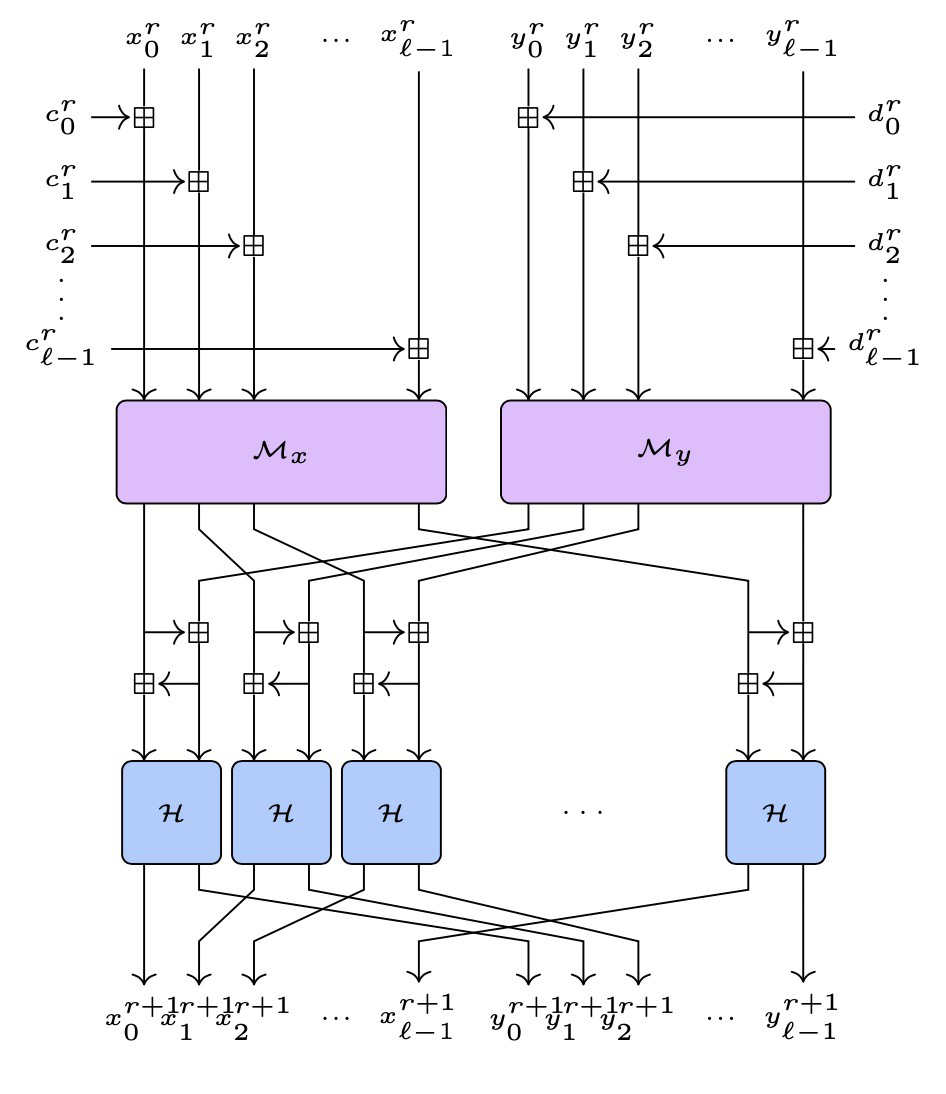
\includegraphics[width=0.8\textwidth]{graphics/anemoi-one-round.png}
    \caption{Round $r$ of Anemoi~\cite{bouvier2023new}}
    \label{fig:anemoi-one-round}
\end{figure}

\subsection*{Anemoi permutation}
The Anemoi permutation, Anemoi$^\pi$ iterates $n_r$ rounds over the round function previously explained, with a linear layer $\mathcal{M}$ when finishing the last round. It is defined as
\begin{equation}
    \text{Anemoi}^\pi_{q,\alpha,l}=\mathcal{M}\circ \text{R}_{n_r-1}\circ\dots \text{R}_0.
\end{equation}
where R$_i$ is the $i$ round function.\\
The number of rounds is computed using $\left(q,\alpha,l\right)$ with
\begin{equation}
    n_r\geq max\{
        8,\text{min}\left(5,1+l\right)+2+\text{min}\{r\in\mathbb{N}|\mathcal{C}_{alg(r)}\geq2^s\}\},
\end{equation}
where
\begin{equation}
    \begin{cases}
        \mathcal{C}_{alg(r)}=\left(\binom{4lr+k_\alpha}{2lr}^2\right) & \text{for } q=p, \\
        \mathcal{C}_{alg(r)}=lr\cdot9^{2lr} & \text{for } q=2^n
    \end{cases}
\end{equation}

\subsection*{Anemoi Hash}
The Anemoi hash function operates over the sponge construction in the field $\mathbb{F}_q^{r+c}$, as all the sponge constructions, $r$ values are used as the rate, and $c$ as the capacity.\\
We must take into consideration that the state has to be separated in $X$ and $Y$ with $l$ elements for each one, so the input must be even.

\subsubsection*{Sponge construction}
There is a modification of the mode of operation of the sponge construction explained in Section~\ref{sec:sponge-construction} and the one used in the Anemoi hash.\\
If we apply the standard sponge construction we may be applying the permutation, Anemoi$^\pi$, one more time when the length of the input is already a multiple of $r$. To solve this, we don't append more blocks at the end of the message if it is a multiple of $r$, rather, we add a constants $\sigma$ before the squeezing phase.\\
This constant $\sigma$ is equal to 0 if the message length is not multiple of $r$, and 1 if it is. Figure~\ref{fig:anemoi-sponge-mod} shows this modification, with $P$ being the Anemoi$^\pi$ permutation.
\begin{figure}[htbp]
    \centering
    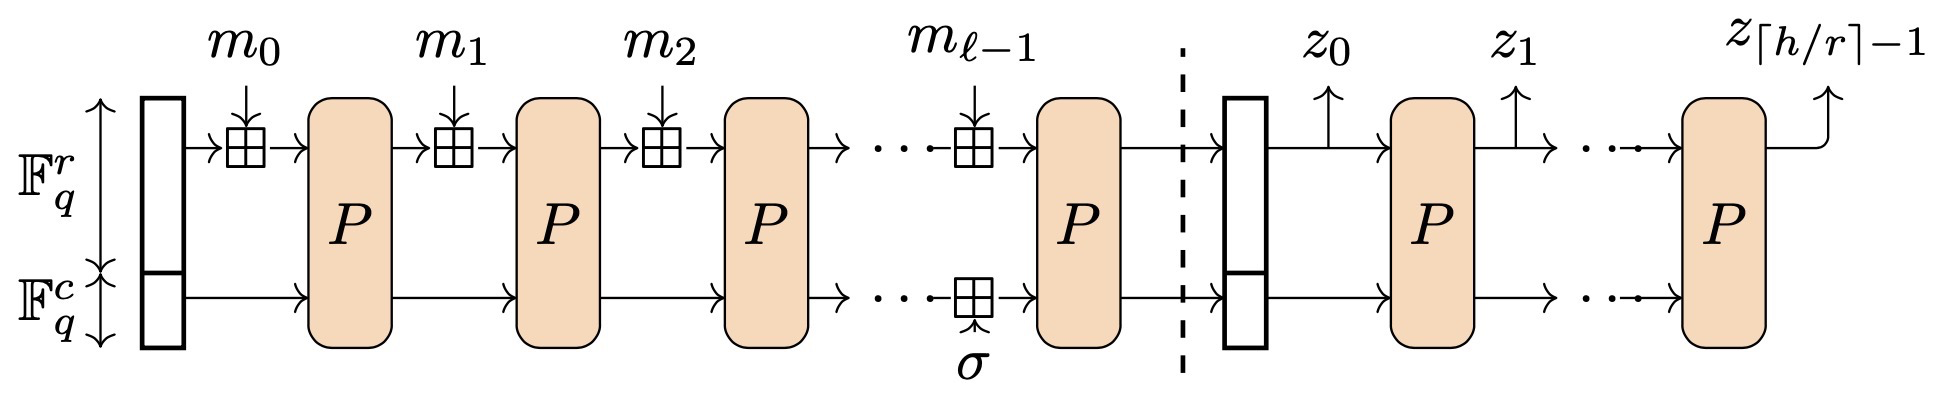
\includegraphics[width=\textwidth]{graphics/anemoi-sponge-mod.png}
    \caption{Anemoi-sponge~\cite{bouvier2023new}}
    \label{fig:anemoi-sponge-mod}
\end{figure}

\section{Arion}
\label{sec:Arion}
The Arion hash function~\cite{roy2023arion} was published by Roy et al. in 2023 and operates over a permutation, and on a lowest level there is the round function.\\
First we are going to explain the round function, followed by the permutation, and finally the hash function.

\subsection*{Arion round funtion}
The Arion hash function works on the $\mathbb{F}_p^t$ vector space, and is defined as
\begin{equation}
    \mathcal{R}_k^{(i)}(x)=\mathcal{K}_k\circ\mathcal{L}_{c_i}\circ\mathcal{F}_{Arion}^{(i)}(x)
\end{equation}

where $\mathcal{R}_k^{(i)}:\mathbb{F}_p^t\times\mathbb{F}_p^t$.

The structure of the Arion round function differs from the previous hash functions, it is composed of the following components: it starts with a GTDS, \textit{Generalized Triangular Dynamical System}~\cite{roy2022generalized}, followed by the affine layer and a keyed permutation.\\
Next, a description of each component is provided below.

\subsubsection*{GTDS Layer}
First, we define a field $\mathbb{F}_p$ with $p$ prime elements. Let $n,d_1,d_2,e\in\mathbb{Z}$ that
\begin{enumerate}
    \item $d_1$ is the smallest positive integer such that gcd$\left(d_1,p-1\right)=1$,
    \item $d_2$ is an integer such that gcd$\left(d_2,p-1\right)=1$,
    \item $e\cdot d_2\equiv1\text{ mod}\left(p-1\right)$. 
\end{enumerate}

The GTDS is defined as $\mathcal{F}_{Arion}=\{f_0,\dots,f_{t-1}\}$ for $1\leq i\leq t-1$, and $\alpha_{i,0},\alpha_{i,1},\beta_i\in\mathbb{F}_p$ so that $\alpha_{i,0}^2-4\cdot\alpha_{i,1}$ is a quadratic non-residue modulo $p$.\\
Thus,
\begin{equation}
    \begin{cases}
        f_i\left(x_0,\dots,x_{n-1}\right)=x_i^d\cdot g_i\left(\sigma_{i+1,t-1}\right)+h_i\left(\sigma_{i+1,t-1}\right), & 0\leq i\leq t-2, \\
        f_{t-1}\left(x_0,\dots,x_{t-1}\right)=x_{t-1}^e, & i=t-1,
    \end{cases}
\end{equation}
where
\begin{align}
    g_i(x)=x^2+\alpha_{i,0}\cdot x+\alpha_{i,1}, \\
    h_i(x)=x^2+\beta_i+x,
\end{align}
and
\begin{equation}
    \sigma_{i+1,t-1}=\sum_{j=i}^{t-1}x_j+f_j\left(x_0,\dots,x_{t-1}\right).
\end{equation}

\subsubsection*{Affine Layer}
The Affine Layer of Arion is defined over the vector space $\mathbb{F}_p^t$ as
\begin{equation}
    \mathcal{L}_c(x)=\text{circ}\left(0,\dots,t-1\right)x+c,
\end{equation}
where circ$\left(0,\dots,t-1\right)$ is the circulant matrix with the first row being $\left(1,\dots,t-1\right)$ and $c\in\mathbb{F}_p^t$ is the constant vector.

\subsubsection*{Keyed permutation}
The keyed permutation, $\mathcal{K}_k$, works over the field $\mathbb{F}_p^t$. It is defined as
\begin{equation}
    \mathcal{K}_k\left(x,k\right)=x+k.
\end{equation}

\subsection*{Arion permutation}
The Arion permutation: $\mathbb{F}_p^t\times\mathbb{F}_p^t\times\left(r+1\right)\rightarrow\mathbb{F}_p^t$ is defined as
\begin{equation}
    \text{Arion}^\pi(x,k_0,\dots,k_{r-1})=\mathcal{R}_{k_{r-1}}^{(r-1)}\circ\dots\circ\mathcal{R}_{k_0}^{(0)}\circ\mathcal{L}_0\circ\mathcal{K}_{k_0}(x)
\end{equation}
for $0\leq i\leq r-1$, where $r$ is the number of rounds of the permutation.\\
Furthermore, the Arion$^\pi$ is instantiated with the key $k_0=\dots=k_{r-1}=0$.

\subsection*{Arion hash}
The Arion hash function works in the field $\mathbb{F}_p^t$ and over the sponge construction. As a sponge construction, the length of the state is $t=r+c$, where $r$ is the rate and $c$ the capacity.